%qqqqqqqqqqqqqqqqqqqqqqqqqqqqqqqqqqqqqqqqqqqqqqqqqqqqqqqqqqqqqqqqqqqqqqqqq
%Quote
\begin{savequote}[50mm]
%‘‘El cosmos es todo lo que es, todo lo que fue y todo lo que será. Nuestras 
%más ligeras contemplaciones del cosmos nos hacen estremecer: Sentimos como 
%un cosquilleo nos llena los nervios, una voz muda, una ligera sensación como
%de un recuerdo lejano o como si cayéramos desde gran altura. Sabemos que nos
%aproximamos al más grande de los misterios.’’
%\qauthor{Carl Sagan}
\end{savequote}
%qqqqqqqqqqqqqqqqqqqqqqqqqqqqqqqqqqqqqqqqqqqqqqqqqqqqqqqqqqqqqqqqqqqqqqqqq




%#########################################################################
%*****************************************************
\chapter{Modelo de Espín.}
\label{cha:Modelo de Spin}
%*****************************************************

El espín\footnote{El espín hace alusión al momentum angular del BH  rotante (Métrica de Kerr)} de BH, es un de los parámetro más relevantes para la dinámica de las galaxias. Este sera el responsable de decir si existe alguna relación entre los AGNs y el entorno que habitan. En esta sección se presentarán los modelos que dan pie al origen, evolución y  alineamiento de los spines.

%===============================================
\section{Agujeros Negros Super Masivos (SMBHs).}
\label{sec: SMBH}
%================================================
Los SMBHs son objetos altamente masivos, que presenta un rango de masas entre $10^6M_{\odot}\lesssim M_{BH} \lesssim 10^{9}M_{\odot}$ \cite{mo2010}. Una de las evidencias que sugiere la existencia de los SMBHs, es que sería el causante de la cantidad de energía que es emitida por los AGNs debido a la acreción de materia (mirar capitulo \ref{sec: Enigma_centarl}). Observaciones en regiones centrales de las galaxias, presentan un incremento en la razón masa-luminosidad, el cual no puede ser explicado por la presencia de poblaciones estelares, a medida que se acerca al centro, la razón masa-luminosidad aumenta, indicando que hay una objeto muy masivo, que no presenta una luminosidad considerable, con lo cual permite postular la existencia de un SMBH, ubicado en la parte central de la galaxia.  

La presencia de un SMBH en la galaxia, solo influye dinámicamente en lugares cercanos a él (centrales). Usando la dispersión de las velocidades para estrellas cercanas al centro es posible encontrar un valor para la masa del objeto central, 

\begin{align}
    r_{BH}=\frac{GM_{BH}}{\sigma^{2}}
\end{align}
donde $\sigma$ es la dispersión de la velocidad, obtenida de medidas observacionales de la cinemática de las estrellas al rededor del cuerpo que gravitan. 

En el contexto cosmológico se considera que todas las galaxias hospedan un SMBH en su interior, muy cercano al centro. Su existencia también viene arraigada por la misma teoría, son consecuencia de la relatividad general y de la teoría de formación de galaxias. 

La importancia de los SMBHs radica es su propiedad de acretar materia convierten en energía, esta energía liberada se conoce como feedback de agujeron negro. Para galaxias grandes, el feedback es el responsable de que la galaxia deje de producir estrellas, debido a que este calienta el gas lo cual impide la formación estelar.

Yendo en dirección de poder conocer la información sobre el spin del BH o SMBH, es necesario poder conocer cómo se origina y evoluciona, es imperioso conocer la teoría que abarca su evolución y su crecimiento.
%------------------------------------------------
\subsection{Crecimiento de SMBHs}
\label{subsec: Crecimiento_SMBHs}
%------------------------------------------------

El proceso de crecimiento de un SMBH esta determinado por la rata de acreción de masa. En la actualidad hay tres maneras posibles para el crecimiento del SMBH: por fusión de BH, colapso de nubes frías de gas que está alrededor galaxia y fusión entre galaxias \cite{fanidakis2011}. Estos tres sucesos pueden dar pie a la formación de AGN, debido a que la activación del AGN es debida por la acreción súbita de materia. 
%-------------------------------------------------------
    \subsubsection{Fusión de BHs}
    \label{subsubsec: mergers_BHs}
%-------------------------------------------------------
La adquisición de materia por fusión entre BHs, corresponde a sistemas  binarios. La fricción dinámica que sienten los BHs  hace que estos pierdan momentum angular, dando como resultando una disminución en la separación entre ellos. También la perdida de energía debido a emisión de las ondas gravitacionales hace que la distancia entre los dos cuerpos se vaya reduciendo, a medida que pasa el tiempo la emisión de las ondas gravitacionales es más consecutiva, haciendo que la perdida de energía sea mayor, dando como resultado la coalescencia entre los dos BHs \cite{fanidakis2011}. 

%-------------------------------------------------------
    \subsubsection{Colapso de nubes de gas}
    \label{subsubsec: colapso_nubes_gas}
%-------------------------------------------------------
En galaxias no muy longevas, donde sea posible encontrar gas frío que esté en inmediaciones del centro de la galaxia, de tal forma que el gas fluye directamente al BHs. Otra manera de acretar gas frio es por medio del metodo de radio-quiet, este mecanismo consiste en que el gas que es expulsado y calentado por la explosiones de supernovas en las galaxias, después de un largo tiempo se enfría y colapsa al centro de la galaxia, donde se encuentra el BH \cite{fanidakis2011}.

%-------------------------------------------------------
    \subsubsection{Colisión de galaxias}
    \label{subsubsec: mergers_galaxys}
%-------------------------------------------------------
La dinámica del universo y las observaciones, dejan ver que la interacción entre galaxias no es en nada extraño, siendo la colisión entre ellas un resultado esperado. Las galaxias espirales en su interior, en especial en la parte más interior del disco presentan una abundancia de gas frio, potencial para: la formación de estrellas, crecimiento de un BH y activación de un AGN. El proceso de fusión entre galaxias se distingue por fusiones mayores y menores\footnote{El proceso de fusión introduce un cambio en la morfología de las galaxias. Si es una fusión menor es posible que no altere la morfología de la galaxia más masiva, de manera considerable; mientras que las fusiones mayores transforma drásticamente la forma de las galaxias. }: las fusiones mayores indica colisiones donde la masa de los dos cuerpos son equivantes, las fusiones menores señala que la diferencia de masas es considerables. Cuando chocan las dos galaxias, ya sea por una fusión mayor o menor, produce un incremento en la formación estelar debido a la acumulación de gas frío de ambas galaxias. Pero no todo el gas frío se transforma en estrellas, parte de este cae al centro alimentando al BH.

%===============================================
\section{Evolución de espín.}
\label{sec: Evolution_spin}
%===============================================

La evolución del espín del SMBH está altamente relacionada con la tasa de acreción de materia por parte del SMBH\cite{king2005}, y por la coalescencia de espines de BHs que colisionan\cite{dubois2014}. Al considerar el interior de un AGN, se tiene entonces una estructura compuesta por un disco de acreción y un SMBH. Al suponer un SMBH rotante, se implica un momentum angular (espín) $\bf{J}_{bh}$, además el disco de acreción también rota y por tanto también posee un momentum angular $\bf{J}_{d}$. Los torques de marea que actúan sobre ambos cuerpos rotantes conduce a alinear los espines, sin cambiar sus magnitudes \cite{king2005}.

El espín del SMBH puede ser definido como ${\bf{J}}_{bh}=|a|GM^{2}_{bh}/c$, donde $a$\footnote{normalizazión del momentum angular del BH.} es el parámetro de spin, acotado entre $-1\leq a \leq 1$. Sí $a=-1$ el BH está rotando en rotando en dirección contraría al disco de acreción, sí $a=1$ el BH y disco rotan en la misma dirección. ${\bf{J}}_{bh}$ juega un papel crucial, para regiones cercanas al BH, indica la eficiencia de convertir la materia del disco en radiación, se cree que también su dirección está relacionada con la dirección del jet de AGN \cite{fanidakis2011}. 

%------------------------------------------------
\subsection{Acreción de gas}
\label{subsec: Acrecion_gas}
%------------------------------------------------
Como se expuso anteriormente, alrededor del SMBH existe un disco de acreción, que es originado por la conservación del momentum angular de las partículas exteriores al disco de acreción. Siguiendo lo propuesto por \cite{lynden1969}, las partículas que se encuentran el disco de acreción pierden momentum angular debido a torques producidos por los campos magnéticos, a medida que se pierden momentum se van adentrando más en el disco, hasta llegar al borde interior del mismo. La orbita más interior es denominada como la ultima orbita estable (del ingles LSO), si la partícula se adentra en esta órbita será devorada por el BH. El radio para la LSO en términos del momentum angular del BH se puede reescribir de la forma \cite{bardeen1972}:
%
\begin{align}
 \hat{r}_{lso}=\frac{r_{lso}}{R_g}=3+Z_{2}\pm \left[ (3-Z_{1})(3+Z_{1}+2Z_{2})\right]^{1/2} \,,
 \label{eq: radio_lso}
\end{align}
%
donde $R_{g}$ es el radio gravitacional, es definido como la mitad del radio de Schwarzchild del BH, 

\begin{align}
    R_{g}= R_{schw}/2  = \frac{GM_{BH}}{c}\,.
\end{align}
De la ecuación (\ref{eq: radio_lso}) se tiene que: para valores de $a<0$ el BH rota de manera contraría a las partículas que estan en la LSO, y si $a>0$ se tiene lo contrario, el BH rota con las partículas. Los parámetros $Z_1$ y $Z_2$ se escriben de la forma:

\begin{eqnarray}
    Z_1 = 1+(1-a^{2})^{1/3}\left[(1+a)^{1/3}+(1-a)^{1/3} \right]\,,\\
    Z_2 = (3a+Z_{1}^{2})^{1/2}\,.
\end{eqnarray}

Un parámetro de gran importancia es la eficiencia radiativa del disco de acreción del BH $\epsilon_{r}$, este parámetro indica cuanta materia se transforma en energía. Al suponer un BH que rota, la eficiencia radiativa dependerá del parámetro de spin $a$ \cite{novikov1973}:
%
\begin{align}
    \epsilon_{r} \equiv 1- \sqrt{1-\frac{2}{3}\frac{1}{\hat{r}_{lso}(a)}}\,,
\end{align}
%
en otras palabras: entre más acreta menos radia ó entre más radia menos acreta.

A medida que el material cae al LSO y posteriormente al BH, conlleva  una emisión de energía por unidad de masa $\widetilde{e}_{lso}$ y un momentum por unidad de masa $\widetilde{l}_{lso}$. Al considerar la masa contenida en región muy cerca a LSO $dM_{0}$, permite calcular el cambio de la masa y del momentum angular del BH, de la forma:
%
\begin{align}
    dM_{BH}=\frac{\widetilde{e}_{lso}}{c^{2}}dM_{0}, \, \, dJ_{BH}=\widetilde{l}_{lso}dM_{0}\,.
    \label{eq: dM_y_dJ}
\end{align}
%
Este ecuación (\ref{eq: dM_y_dJ}) se relaciona con la ecuación para el espín del BH total ${\bf{J}}_{BH}$ de la forma:
%
\begin{align}
    \frac{da}{d\ln{M_{BH}}}=\frac{1}{M_{BH}}\frac{c^{3}}{G}\frac{\widetilde{l}_{lso}}{\widetilde{e}_{lso}}-2\,,
\end{align}
%
La integral a esta solución es obtenida por \cite{bardeen1970}, dando como resultado: 
\begin{align}
    a^{f}=\frac{1}{3}\hat{r}_{lso}^{2}\frac{M_{BH}}{M_{BH}^{f}}\left[1- \left\{3\hat{r}_{lso}\left(\frac{M_{BH}}{M^{f}_{BH}} \right)^{2}-2 \right\}^{1/2} \right]\,,
    \label{eq: espin_final a^f}
\end{align}
donde $a^{f}$ y $M_{BH}^{f}$, corresponden al espín y masa final del BH. La ecuación (\ref{eq: espin_final a^f}) determina la evolución del espín $a$ durante el tiempo de acreción para un estado inicial. 

\begin{center}
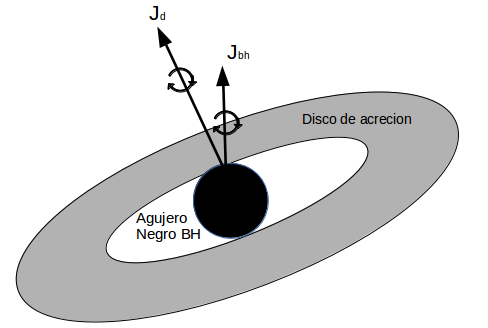
\includegraphics[scale=.35]{./figures/4_Modelo_Spin/Modelo_disco_bh.png}
\figcaption{\emph{Modelo donde se muestra que el disco de acreción y el BH están desalineados.}}\label{fig: desaliniamineto_bh_disco}
\end{center}

%------------------------------------------------
    \subsubsection{Acreción de gas en discos desalineados}
    \label{subsubsec: Acrecion gas desaliniado}
%------------------------------------------------
Siguiendo lo anteriormente expuesto, se tiene un disco de acreción que orbita alrededor de un BH. Los dos sistemas al estar rotando presentan un momemtum angular ${\bf{J}}_{bh}$ y ${\bf{J}}_{d}$. Gracias al análisis y resultados en \ref{subsec: Acrecion_gas} es posible asumir que la evolución del espín del BH, depende de la Masa acretada por el mismo, ecuación (\ref{eq: espin_final a^f}). El proceso de acreción y cantidad de masa acomulada trasciende el análisis que se pretende realizar, sin embargo es posible tener un estimativo de estos procesos, a partir de los que sigue. Al considera el caso más general donde se tiene el disco de acreción rota en un plano diferente al plano ecuatorial del disco, (ver figura \ref{fig: desaliniamineto_bh_disco}). Al considerar este sistema se tiene entonces, que el disco de acreción genera un torque debido al efecto Lense-Thirring (LT) producto de la rotación del BH. El efecto LT puede ser puede ser escrito de la forma:
%
\begin{align}
    \frac{\partial {\bf{L}}}{\partial t}={\bf{\Omega}}_{p}\times{\bf{L}}\,,
    \label{eq: lense-Thirring}
\end{align}
%
donde ${\bf{L}}$ es el momentum angular por unidad de area del disco y ${\bf{\Omega}}_{p}$ es rata de preseción, definida de la forma:
%
\begin{align}
    {\bf{\Omega}}_{p}=\frac{2G}{c}\frac{{\bf{J}}_{bh}}{R^{3}}\,,
\end{align}
%
donde $R$ es la distancia al BH \cite{pringle1992}. La viscosidad del disco determina altamente la evolución de los espines, entre más grande sea la viscosidad de las partículas en el disco es menor su tiempo de alineación, además si es lo suficientemente alta, las partículas del interior generan otro disco que se alinea con el espín del BH. Entonces, es necesario introducir las escalas de tiempo que brindan información importante de la dinámica del sistema: Se introduce el tiempo de escala de acreción $t_{acc}\equiv R^{2}/\nu_{1}(R)$, indicando el tiempo que demora las partículas del disco en caer al BH de manera paralela, el tiempo de escala warp $t_{warp}\equiv R^{2}/\nu_{2}(R)$, que equivale al tiempo de propagación de la deformación en dirección normal.  

Sin embargo ese disco warp\footnote{disco interno que fue deformado por la alta viscosidad} deformado no mantiene la misma dirección, este precesa al rededor del plano ecuatorial de BH. El tiempo de precesión esta definido como:
%
\begin{align}
    t_{prec}= \frac{2\pi}{{\bf{\Omega}}_p(R)}
\end{align}





%------------------------------------------------
    \subsubsection{Alineamiento o contra-alineamiento del espín}
    \label{subsubsec: Aling_Spin}
%------------------------------------------------











%*************************************************************************